%%% License: Creative Commons Attribution Share Alike 4.0 (see https://creativecommons.org/licenses/by-sa/4.0/)
%%% Slides are based heavily on earlier versions of this course taught by Jesper Rudiger.

\documentclass[english,10pt
%,handout
,aspectratio=169
]{beamer}
%%% License: Creative Commons Attribution Share Alike 4.0 (see https://creativecommons.org/licenses/by-sa/4.0/)
%%% Slides are based heavily on earlier versions of this course taught by Jesper Rudiger and Peter Norman Sorensen.

\DeclareGraphicsExtensions{.eps, .pdf,.png,.jpg,.mps,}
\usetheme{reMedian}
\usepackage{parskip}
\makeatother

\renewcommand{\baselinestretch}{1.1} 

\usepackage{amsmath, amssymb, amsfonts, amsthm}
\usepackage{enumerate}
\usepackage{hyperref}
\usepackage{url}
\usepackage{bbm}
\usepackage{color}

\usepackage{tikz}
\usepackage{tikzscale}
\newcommand*\circled[1]{\tikz[baseline=(char.base)]{
		\node[shape=circle,draw, inner sep=-20pt] (char) {#1};}}
\usetikzlibrary{automata,positioning}
\usetikzlibrary{decorations.pathreplacing}
\usepackage{pgfplots}
\usepgfplotslibrary{fillbetween}
\usepackage{graphicx}

\usepackage{setspace}
%\thinmuskip=1mu
%\medmuskip=1mu 
%\thickmuskip=1mu 


\usecolortheme{default}
\usepackage{verbatim}
\usepackage[normalem]{ulem}

\usepackage{apptools}
\AtAppendix{
	\setbeamertemplate{frame numbering}[none]
}
\usepackage{natbib}



\title{Financial Markets Microstructure \\ Lecture 5}

\subtitle{Glosten-Milgrom Model\\
	Chapter 3.3 of FPR}

\author{Egor Starkov}

\date{K{\o}benhavns Unversitet \\
	Spring 2022}



\begin{document}
	\AtBeginSection[]{
		\frame<beamer>{
			\frametitle{This lecture:}
			\tableofcontents[currentsection,currentsubsection]
	}}
	\frame[plain]{\titlepage}


\begin{frame}{What did we do last time?}
\begin{enumerate}
	\item Argued that market thinness is not the only source of illiquidity
	\item Poked holes in the Efficient Market Hypothesis
	\item Defined price efficiency in many ways
	\item Began talking about the GM model
\end{enumerate}
\end{frame}


\begin{frame}{Today}
\begin{enumerate}
	\item more Glosten-Milgrom!
\end{enumerate}
\end{frame}


\section{Glosten-Milgrom}

\begin{frame}{GM85: Overview}
	\begin{itemize}
		\item Dynamic model, periods $t = 1,2,...$
		\item Two players in every period:
		\begin{itemize}
			\item trader and dealer
			\item \alert{dealer} long-lived; trader new every period
			\item \alert{trader} can be informed or not
		\end{itemize}
	\end{itemize}
\end{frame}


\begin{frame}{GM85: Model (1)}
	\textbf{Trader:} is either a speculator or a noise trader, can submit a market order to buy or sell one unit of the asset.
	\begin{itemize}
		\item \structure{Speculator} (probability $\pi$): has private information.
		\begin{itemize}
			\item Risk neutral, chooses his market order $d$ to maximize expected profits:
			\begin{equation*}
				d_t= \left\{
				\begin{aligned}
				1	& \text{ if buy}; \\
				0	& \text{ if abstain}; \\
				-1	& \text{ if sell}.
				\end{aligned}
				\right.
			\end{equation*}
			\item `Hides' behind noise traders
		\end{itemize}
		\item \structure{Noise trader} (probability $1-\pi$): trades for exogenous reasons (hedging, liquidity).
		\begin{itemize}
			\item Buys with fixed probability $\beta_B$; sells w.p. $\beta_S$; abstains w.p. $1-\beta_B - \beta_S$
			\item \alert{Important}: we often assume that these traders behave in a certain way (behavior types) but they can be perfectly rational!
		\end{itemize}
	\end{itemize}
\end{frame}


\begin{frame}{GM85: Model (2)}
	\textbf{Dealer (market maker)}
	\begin{itemize}
		\item Risk neutral
		\item Willing to trade \alert{exactly one unit} (buy/sell/no trade) each period
		\item Sets \alert{bid and ask prices} (for a single unit)
		\item Quote price before seing trade (limit order)
		\item Does not know whether trader is speculator or noise trader
		\item \structure{Competitive}: prices=expected asset value conditional on information
		\item Trading is sequential: market orders served one by one
	\end{itemize}
\end{frame}


\begin{frame}{GM85: Model (3)}
\begin{itemize}
	\item \textbf{Asset value}:
	\begin{itemize}
		\item Random asset value $v$ drawn from distribution
		\item Assume $v$ is the fundamental (terminal) value
		\item Speculators know $v$ perfectly (not much changes if they don't)
	\end{itemize}
	\item \textbf{Equilibrium}:
	\begin{itemize}
		\item An equilibrium consists of \structure{bid and ask prices} and \structure{speculator's strategy}
		\item They must be such that: (i) prices are competitive (zero profit for MM), (ii) speculator best-responds to prices (maximizes expected gain).
	\end{itemize}
\end{itemize}
\end{frame}


\begin{frame}{Some questions}
\begin{itemize}%[<+->]
	\item Why are there no uninformed speculators?
	\item What is the role of the dealer? What functions does he fulfill?
	\item Why is the dealer willing to trade with better-informed speculators?
\end{itemize}
\end{frame}


\begin{frame}{Analysis. A: Market making}
\begin{itemize}%[<+->]
	\item Dealer quotes bid and ask prices on \textit{one unit}
	\begin{itemize}
		\item Can revise prices between each incoming trade
	\end{itemize}
	\item Quoted ask price $a_t$ only relevant if next incoming trader decides to buy
	\begin{itemize}
		\item Same for bid $b_t$
	\end{itemize}
	\item Risk neutrality and competition implies that the \structure{ask price} and \structure{bid price} are
	\begin{align*}
		a_t & = \mathbb{E}[v|\Omega_{t-1}, Buy]; \\
		b_t &= \mathbb{E}[v|\Omega_{t-1},  Sell].
	\end{align*}
	\item Notice that both sides of the equality depend on prices
\end{itemize}
\end{frame}


\begin{frame}{Analysis. B: Informed trading}
\begin{itemize}
	\item Speculator knows $v$. Given prices $a_t$ and $b_t$, the expected profits $\Pi$ are:
	\begin{equation*}
		\Pi(v,a_t,b_t,d_t)= \left\{
		\begin{aligned}
		&v - a_t  	&& \text{ if } d_t=1; \quad && (Buy)\\
		&0			&&\text{ if } d_t=0; \quad && (Abstain)\\
		&b_t - v 	&& \text{ if } d_t=-1. \quad && (Sell)
		\end{aligned}
		\right.
	\end{equation*}
	\pause
	\item Speculator's best response to $(a_t,b_t)$ is: (assume $a_t \geq b_t$)
	\begin{itemize}
		\item Buy when $v > a_t$, i.e. when $v$ is large enough
		\item Sell when $v<b_t$, i.e. when $v$ is small enough
		\item Abstain if $a_t > v > b_t$
	\end{itemize}
\end{itemize}
\end{frame}


\begin{frame}{Analysis. C: Equilibrium definition}
Dealer must make zero profit ({competition}), traders must trade optimally.
This gives us two \structure{equilibrium conditions}.
\begin{itemize}
	\item Let $\sigma_t$ denote the speculator's strategy, where $\sigma_t(d_t|v)$ is the probability that the speculator places order $d_t$ if value is $v$
	\item \alert{An equilibrium} consists of \structure{prices $(a_t,b_t)$} and \structure{strategy $\sigma_t$} such that:
	\begin{enumerate}
		\item the ask and bid prices  solve 
		\begin{align*}
		a_t & = \mathbb{E}[v| \Omega_{t-1}, Buy]; \\
		b_t & = \mathbb{E}[v| \Omega_{t-1}, Sell],
		\end{align*}
		given $\sigma_t$
		\item for each $v$, $\sigma_t$ solves 
		\[
		\max_{\sigma_t } \, \{\sigma_t(1|v) [v-a_t] + \sigma_t(-1|v)[b_t-v] \},
		\]
		given $(a_t,b_t)$.
	\end{enumerate} 
\end{itemize}
\end{frame}


\begin{frame}{Back to homework}
	\begin{exampleblock}{GM Example}
		\begin{itemize}
			\item \textbf{Single period}: Suppose only one period (drop $t$ subscript, drop $\Omega$)
			\item \textbf{Binary outcome}: $v \in \{ 0, 1\}$, equally likely ex ante: $\mathbb{P}(v=1) = 0.5$.
			\item Suppose $0 < b < a < 1$ and noise trader's order obeys $\beta_B=\beta_S=0.5$. 
		\end{itemize}
		Questions:
		\begin{enumerate}
			\item What is the speculator's trading strategy?
			\item Can you derive dealer's \alert{prices $a$ and $b$}, as a function of $\pi$?
			\begin{itemize}
				\item If not, refresh your knowledge of conditional expectations and try again.
				\item If you already read the solution in the book, try to replicate it without looking back at the book.
			\end{itemize}
			\item Are the resulting prices efficient? (Check all three forms)
		\end{enumerate}
	\end{exampleblock}
\end{frame}


\begin{frame}{Analysis. D: Solving for equilibrium (1)}
	\begin{itemize}
		\item The orders reveal information about $v$. E.g., a \alert{buy order} is submitted:
		\begin{itemize}
			\item either by a noise trader (probability $(1-\pi)\beta_B$) -- no new information, $\mu_t = \mu_{t-1} = \mathbb{E}[v|\Omega_{t-1}]$;
			\item or by a speculator (probability $\pi \mathbb{P}(v \geq a_t | \Omega_{t-1})$) -- then learn that $v \geq a_t$, so $\mu_t = \mathbb{E} [v | \Omega_{t-1}, v \geq a_t]$.
		\end{itemize}
		\item Then $a_t$ is given by (using Bayes' rule and law of total probability):
		\visible<handout:0|2->{
		\begin{align*}
			a_t &= \mathbb{E}[v|\Omega_{t-1}, Buy]
			\\
			= \frac{\mathbb{P}(Buy,Noise|\Omega_{t-1}, v)}{\mathbb{P}(Buy|\Omega_{t-1}, v)} \cdot \mathbb{E}[v|\Omega_{t-1}] &+ \frac{\mathbb{P}(Buy,Informed|\Omega_{t-1}, v)}{\mathbb{P}(Buy|\Omega_{t-1}, v)} \cdot \mathbb{E} [v | \Omega_{t-1}, v \geq a_t]
			\\
			= \frac{(1-\pi)\beta_B}{(1-\pi) \beta_B + \pi \mathbb{P}(v \geq a_t)} \cdot \mu_{t-1} &+ \frac{\pi \mathbb{P}(v \geq a_t | \Omega_{t-1})}{(1-\pi) \beta_B + \pi \mathbb{P}(v \geq a_t)} \cdot \mathbb{E} [v | \Omega_{t-1}, v \geq a_t],
		\end{align*}
		}
		meaning that in the end, $a_t \geq \mu_{t-1}$.
	\end{itemize}
\end{frame}


\begin{frame}{Analysis. D: Solving for equilibrium (2)}
	\begin{itemize}
		\item Similarly for \alert{sell orders}:
		\begin{itemize}
			\item sell order from a noise trader arrives with [unconditional] probability $(1-\pi)\beta_S$ -- no new information, $\mu_t = \mu_{t-1}$;
			\item sell order from a speculator arrives with probability $\pi \mathbb{P}(v \leq b_t | \Omega_{t-1})$ -- then learn that $v \leq b_t$, so $\mu_t = \mathbb{E} [v | \Omega_{t-1}, v \leq b_t]$.
		\end{itemize}
		\item Then $b_t$ is given by:
		\visible<handout:0|2->{
		$$ b_t = \mathbb{E}[v|\Omega_{t-1}, Sell] $$
		$$ = \frac{(1-\pi)\beta_S}{\mathbb{P}(Sell|\Omega_{t-1}, v)} \cdot \mathbb{E}[v|\Omega_{t-1}] + \frac{\pi \mathbb{P}(v \leq b_t | \Omega_{t-1})}{\mathbb{P}(Sell|\Omega_{t-1}, v)} \cdot \mathbb{E} [v | \Omega_{t-1}, v \leq b_t] $$}
		\begin{itemize}
			\visible<handout:0|2->{
			\item where $\mathbb{P}(Sell|\Omega_{t-1}, v) = (1-\pi) \beta_S + \pi \mathbb{P}(v\leq b_t)$,
			}
			\item so $b_t \leq \mu_{t-1}$, and we have confirmed that indeed $a_t \geq b_t$.
		\end{itemize}
	\end{itemize}
\end{frame}


\begin{frame}{Analysis. E: Price efficiency}
	\begin{itemize}
		\item $\mu_t \equiv \mathbb{E}[v | \Omega_t]$ is the expectation of $v$ \textit{after} the time-$t$ trade order is observed. Note that in our model:
		$$\mu_t = \begin{cases}
			a_t & \text{ if buy order at } t;
			\\
			b_t & \text{ if sell order at } t.
		\end{cases} $$
		\item Meaning market price is efficient: $p_t = \mu_t$
		\begin{itemize}
			\item in \alert{semi-strong} form,
			\item not in the \alert{strong} form (equivalent to $p_t = v$)
		\end{itemize}
		\item This is because dealers are \structure{competitive}
		%\item let $s^a_t = a_t - p_t$ and $s^b_t = b_t - p_t$ denote the `half-spreads'.
	\end{itemize}
\end{frame}



%\iffalse 

\section{GM example}

\begin{frame}{Example (as in book)}
\begin{itemize}
	\item \textbf{Single period}: Suppose only one period (drop $t$ subscript, drop $\Omega$)
	\item \textbf{Binary outcome}: $v \in \{ v^H, v^L\}$, with prior $\theta=\mathbb{P}(v^H) $ 
	\item \textbf{Prior value}: What is the prior value of the asset before trading?
	\[
	\mu=\theta v^H+(1-\theta) v^L.
	\]
	\hyperlink{overview}{\beamerbutton{Skip example}}
\end{itemize}
\end{frame}


\begin{frame}{Example (2)}
	\begin{itemize}
		\item How do we solve the model? Look for equilibrium with trade. 
		\item Suppose $v^L < b < a < v^H$.
		\item Then speculator buys if $v=v^H$, sells if $v=v^L$. 
		\begin{itemize}
			\item That is, $\sigma(1|v^H)=1$ and $\sigma(-1|v^L)=1$
		\end{itemize}
		\item The procedure is then the following
		\begin{enumerate}
			\item Use the equilibrium conditions from before to calculate prices given the above speculator strategy
			\item Check that these prices satisfy $v^L < b < a < v^H$
		\end{enumerate}
	\end{itemize}
\end{frame}


\begin{frame}{Example (3)}
\begin{itemize}
	\item Let's solve for the ask price. First:
	\begin{align*}
		\mathbb{P}(Buy| v^H) & = (1-\pi) \beta_B + \pi \\
		\mathbb{P}(Buy| v^L) & = (1-\pi) \beta_B
	\end{align*}
	Then by Bayes' Rule
	\begin{align*}
		\mathbb{P}(v^H|Buy) & = \frac{\mathbb{P}(v^H) \mathbb{P}(Buy| v^H)}{\mathbb{P}(Buy)}  \\
		& = \frac{\theta [(1-\pi)\beta_B+\pi]}{(1-\pi)\beta_B+ \pi\theta}  \\
		& =  \theta + \frac{\theta(1-\theta) \pi}{(1-\pi)\beta_B+\pi\theta}
	\end{align*}
\end{itemize}
\end{frame}


\begin{frame}{Example (4)}
\begin{itemize}
	\item The ask price is the expected value, given a buy order:
	\begin{align*}
		a 
		& = \mathbb{P}(v^H| Buy) v^H + [1-\mathbb{P}(v^H| Buy)] v^L \\
		& = \left[ \theta + \frac{\theta(1-\theta) \pi}{(1-\pi)\beta_B+\pi\theta} \right] v^H + \left[ 1 - \left( \theta + \frac{\theta(1-\theta) \pi}{(1-\pi)\beta_B+\pi\theta} \right) \right] v^L\\
		& = \mu + \frac{\theta(1-\theta) \pi}{(1-\pi)\beta_B+\pi\theta} (v^H -v^L).
	\end{align*}
	\item Doing a similar exercise for $b$ we find
	\begin{align*}
		b 		&= \mu - \frac{\theta(1-\theta) \pi}{(1-\pi)\beta_S+\pi(1-\theta)}(v^H-v^L)
	\end{align*}
	\item Finally, we must check that our assumption holds: easy to check that $v^H > a > b > v^L$. Hence, \alert{this is an equilibrium}
\end{itemize}
\end{frame}


\begin{frame}{Example: Lessons}
	\begin{align*}
	a - \mu 		&= \frac{\theta(1-\theta) \pi}{(1-\pi)\beta_B+\pi\theta}(v^H-v^L) \\
	\mu - b 		&= \frac{\theta(1-\theta) \pi}{(1-\pi)\beta_S+\pi(1-\theta)}(v^H-v^L)
	\end{align*}
	\begin{itemize}
		\item Add the two expressions to get bid-ask \structure{spread} $S = a-b$
		\begin{itemize}
			\item $S$ \alert{increases in $\pi$}: more informed trading exacerbates adverse selection. Opposite for $(\beta_B+\beta_S)$.
			%NOTE: monotonicity in pi verified, difficult to compute
			\item If $\beta_B=\beta_S=1/2$, $S$ is \alert{increasing in $\theta(1-\theta)$}, i.e. spread higher when dealer faces greater initial uncertainty about $v$. Same for $(v^H-v^L)$.
		\end{itemize}
	\end{itemize}
\end{frame}


%\begin{frame}[label=insights]{Insights}
%	\begin{itemize}
%		\item Are prices efficient here? What kind of efficiency?
%		\hyperlink{efficiency}{\beamerbutton{Efficiency}}
%		\item What is the effect of speculators (insider traders)?
%		\hyperlink{insiders}{\beamerbutton{Insiders}}
%		\item The effect of price volatility ($v^H - v^L$)
%		\hyperlink{volatility}{\beamerbutton{Volatility}}
%		\item What's the effect of trading frequency? (How can we think about it here?)
%		\hyperlink{frequency}{\beamerbutton{Frequency}}
%		\item What is the dealer's profits? What about the speculators?
%		\hyperlink{profits}{\beamerbutton{Profits}}
%	\end{itemize}
%\end{frame}


\begin{frame}[label=example]{Example: Price discovery}
\begin{itemize}
	\item Return to the multiperiod setting. One unit traded every period, $v$ persistent.
	\item Trade flow is \alert{informative} -- trades have long-lasting effect on prices
	\item Each order conveys information, dealers learn, and 
	$$p_t \rightarrow v \quad
	\hyperlink{dynamics}{\beamerbutton{Dynamics}} $$
	prices \alert{strong-form efficient} in the long run
	\pause
	\item Speed of price discovery increasing in $\pi$
	\begin{itemize}
		\item Trade-off between \structure{price discovery} and \structure{liquidity}
	\end{itemize}
\end{itemize}
\end{frame}


\begin{frame}{Example: Simulation}
	Dealer beliefs: Each curve shows the evolution of dealer's beliefs in each run (10 runs of 100 orders)
	\quad
	\center
	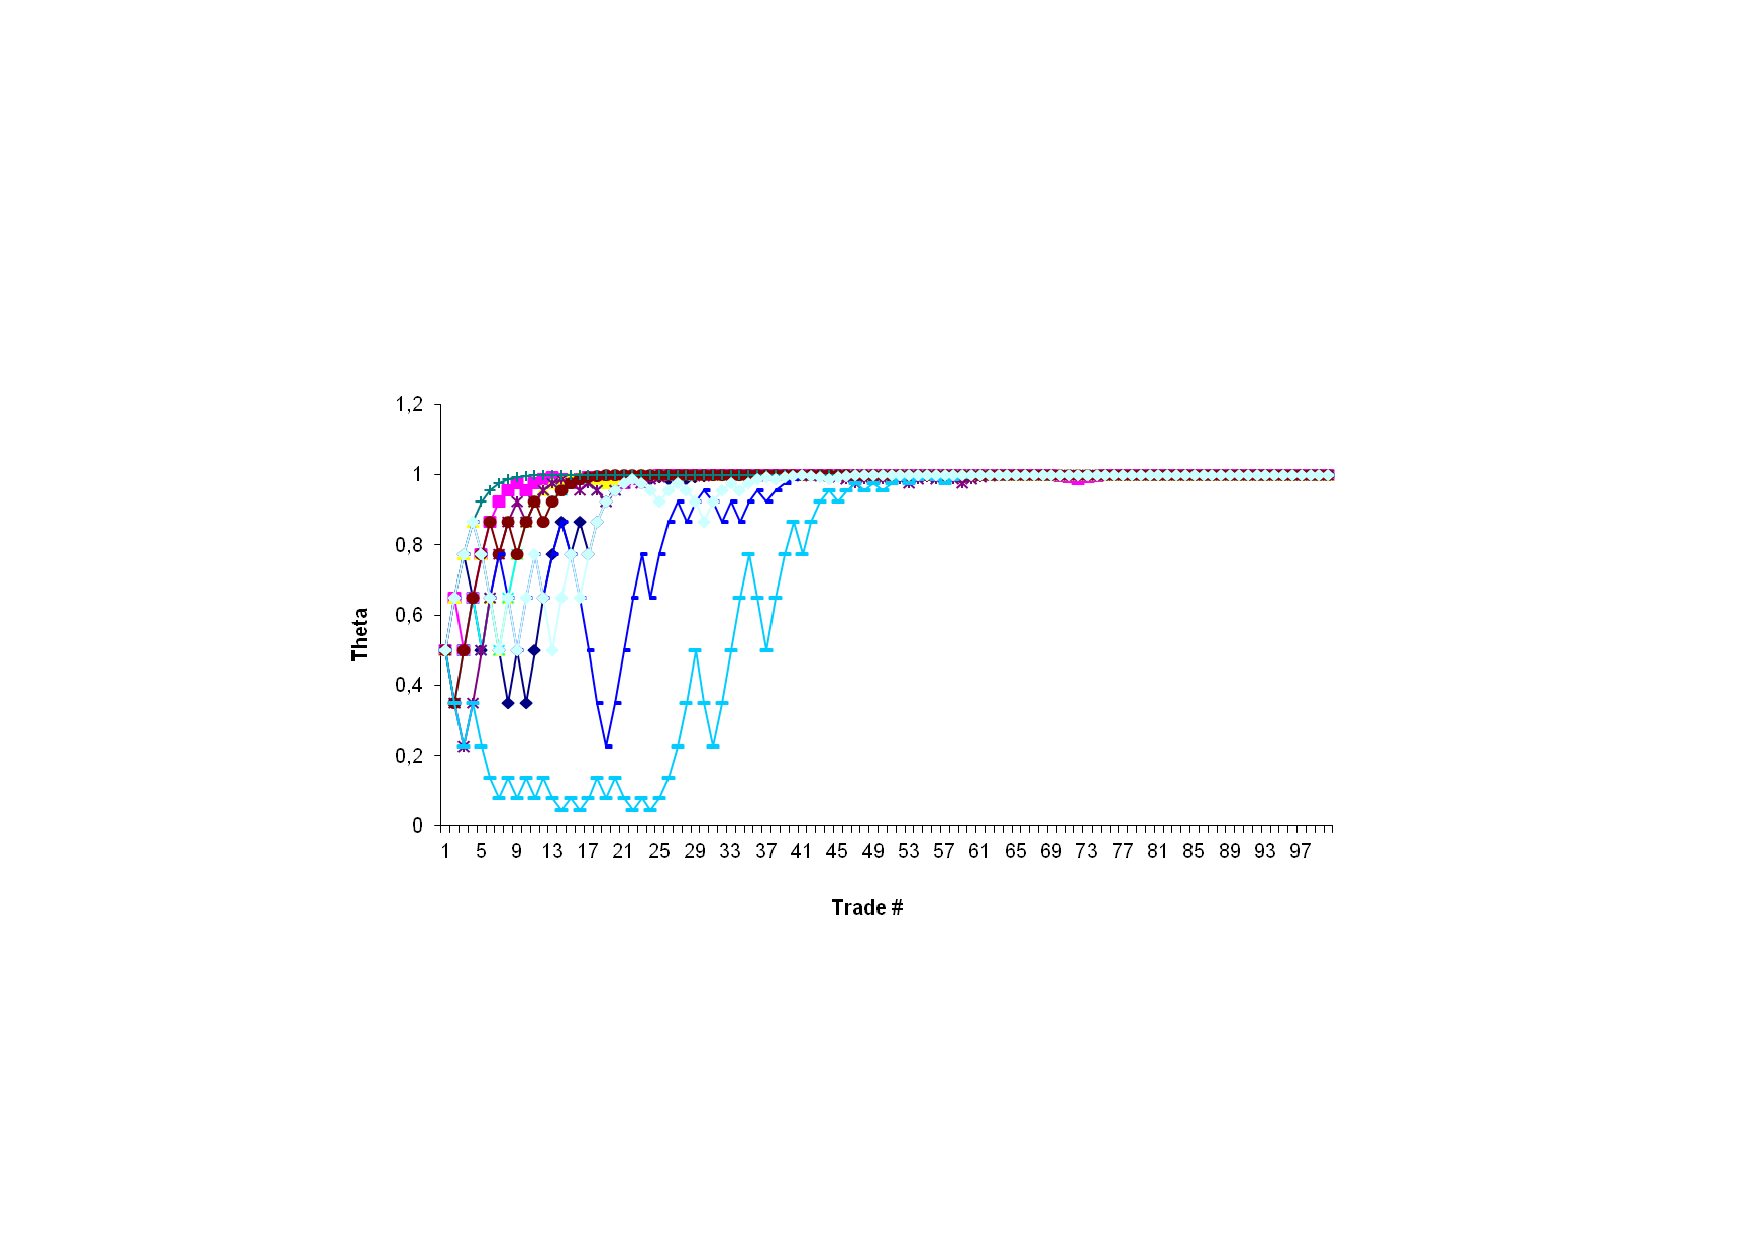
\includegraphics[width=0.95\linewidth]{pics/DealerBeliefs_Image.pdf}
\end{frame}


\section{GM: conclusions}

\begin{frame}[label=overview]{Model overview: Glosten and Milgrom}
	\structure{Model}
	\begin{itemize}
		\item \textbf{Dealer model}: Prices are set each period, discriminative, normally competitive (zero profits)
		\item \textbf{Non-market clearing}: Only one unit traded  - not market clearing (traders may wish to buy/sell more)
		\item Only \textbf{fundamental value} matters,  no speculation/resale
	\end{itemize}
	\structure{Discussion}
	\begin{itemize}
		\item \textbf{Insights}: Adverse selection as a driver of the spread
		\item \textbf{Shortcomings}: Trade fixed amount, trade once, no resale
		\item \textbf{Advantages}: (Relatively) simple analysis, flexible %, trader is not price-taker (realizes price-impact)
	\end{itemize}
\end{frame}


\begin{frame}{Summary}
	What did we learn from the Glosten and Milgrom model?
	\begin{enumerate}
		\item Information, prices and the spread
		\begin{itemize}
			\item Prices will reflect the information revealed by trades
			\item The spread is increasing in informational asymmetry (adverse selection) and in uncertainty about asset value
		\end{itemize}
		\item Informational efficiency
		\begin{itemize}
			\item Prices are always semi-strong efficient, in the long run also strong-form efficient
		\end{itemize}
		\item Noise trading
		\begin{itemize}
			\item Noise trading keeps the market liquid and improves spreads
			\item Informed speculation increases spreads, but improves price discovery - dilemma for regulators
		\end{itemize}
	\end{enumerate}
\end{frame}


\begin{frame}{Homework}
	\begin{itemize}
		%\item See a text from The Securities and Exchange Commission on insider trading, from its homepage \url{http://www.sec.gov/answers/insider.htm}. Discuss potential restrictions in the definition.
		\item Reading:
		\begin{itemize}
			\item Read two articles on absalon on how ESMA restricted trading and binary options and SEC restricted trading in certain stocks.
			\item What is the difference between the underlying assets in the two cases?
			\item Explain ESMA's decision using GM model.
		\end{itemize}
		\item Solving:
		\begin{itemize}
			\item FPR chapter 3, exercise 3 (GM model where speculators are not perfectly informed, but instead receive a signal about the value of the asset)
			\item GM example with $v \sim U[0,1]$ (rest as in the problem assigned before today; goal: derive the equilibrium bid and ask prices)
		\end{itemize}
	\end{itemize}
\end{frame}


\section{extras}

\begin{frame}[label=dynamics]{Dynamics}
	Suppose we are in the simple binary model with the following parameters
	\begin{itemize}
		\item Probability of informed speculators: $\pi = 0.3$
		\item Probability (ex ante) of high value: $\theta = 0.5$
		\item $v^H=150$ and $v_L=100$
	\end{itemize}
	Consider 12 periods, with the following sequence of buys (b) and sells (s)
	\[
	ssbssssssssss
	\]
\end{frame}


\begin{frame}<handout:0>{Dynamics}
	First period: sell
	\center
	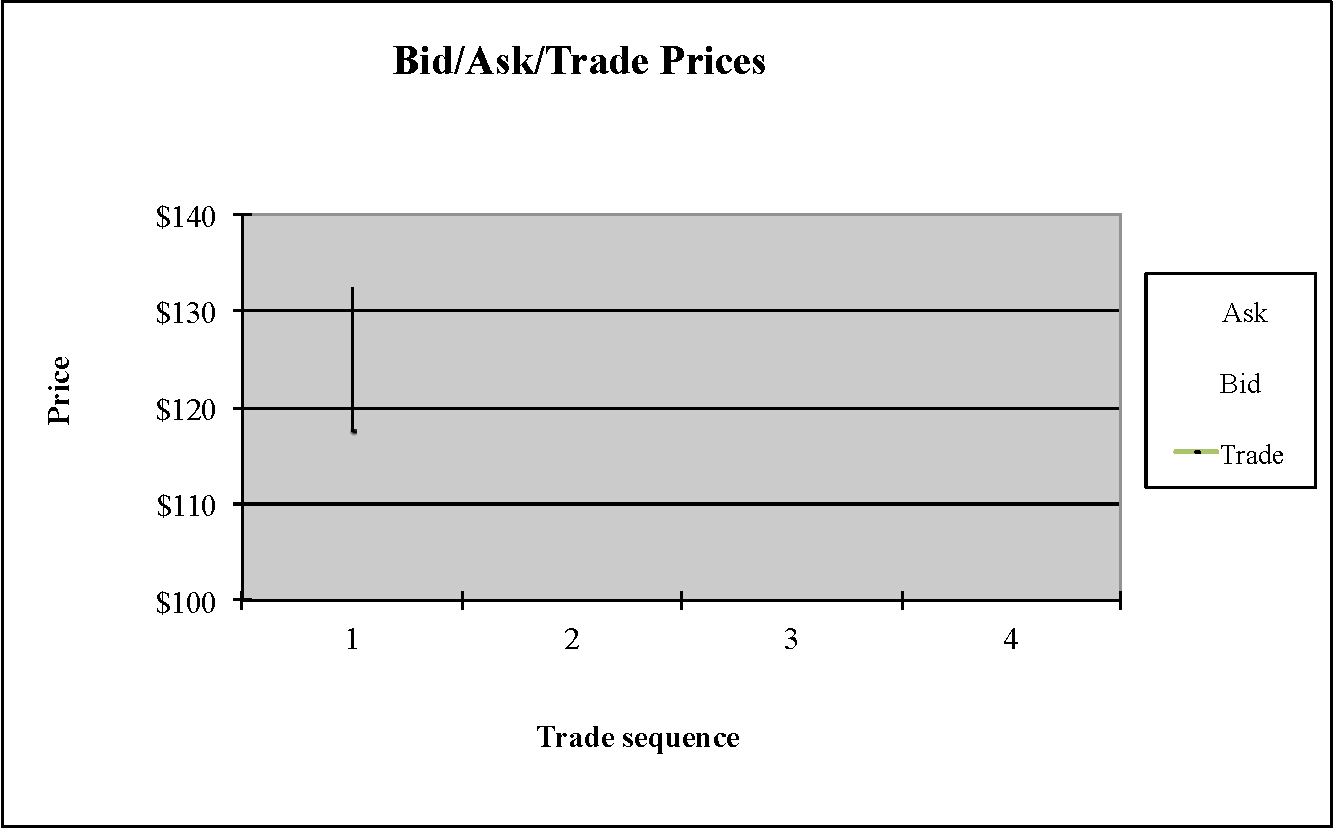
\includegraphics[width=0.9\linewidth]{pics/P1_Image.pdf}
\end{frame}


\begin{frame}<handout:0>{Dynamics}
	Second period: sell
	\center
	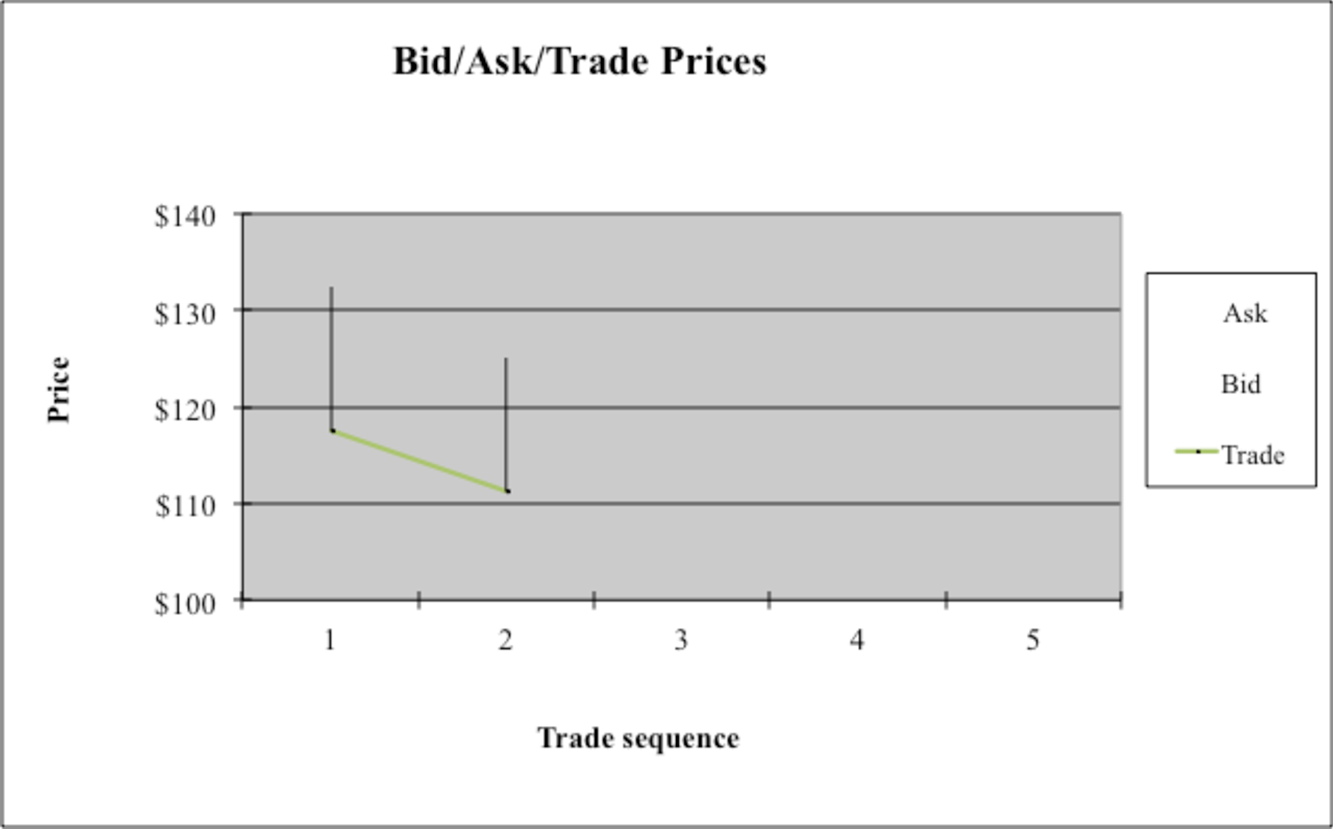
\includegraphics[width=0.9\linewidth]{pics/P2_Image.pdf}
\end{frame}


\begin{frame}<handout:0>{Dynamics}
	Third period: buy
	\center
	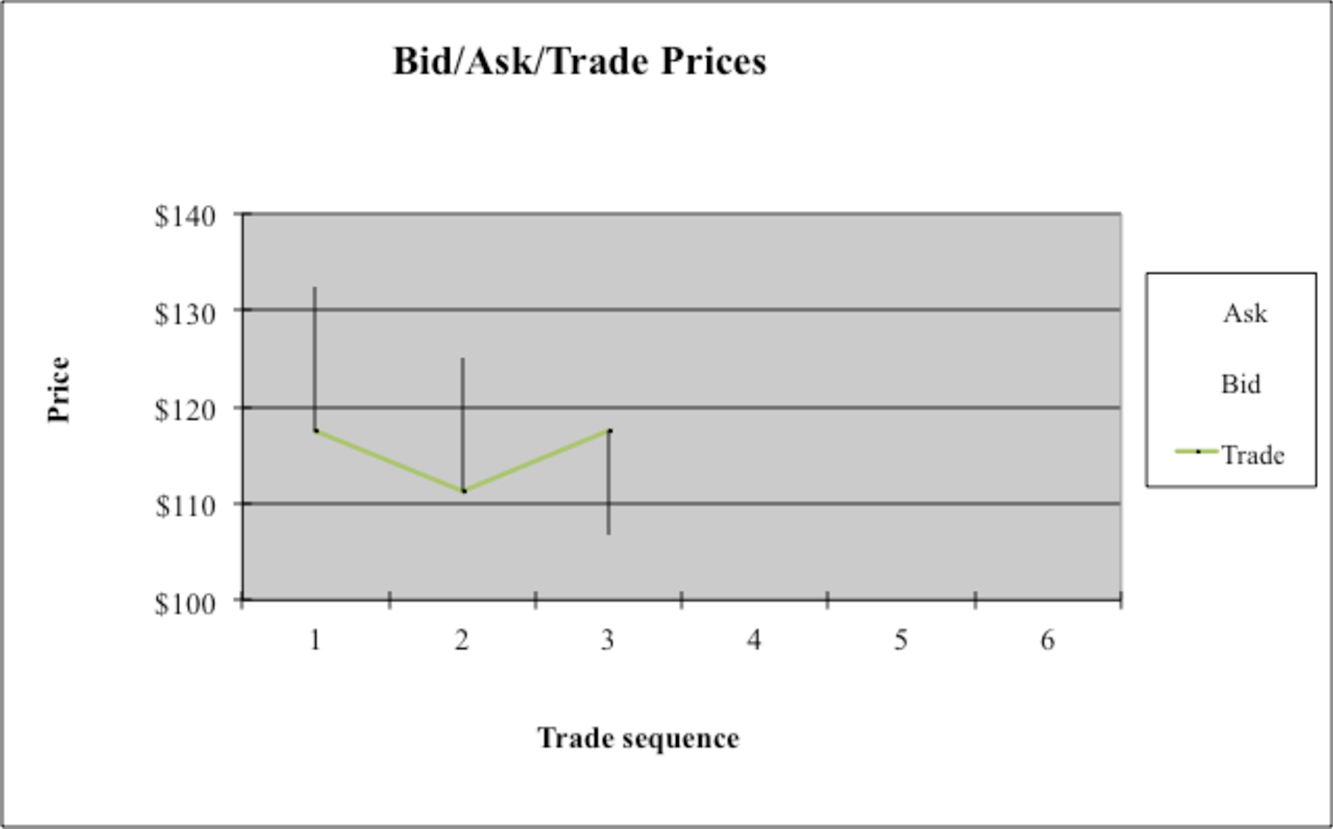
\includegraphics[width=0.9\linewidth]{pics/P3_Image.pdf}
\end{frame}


\begin{frame}<handout:0>{Dynamics}
	Fourth period: sell
	\center
	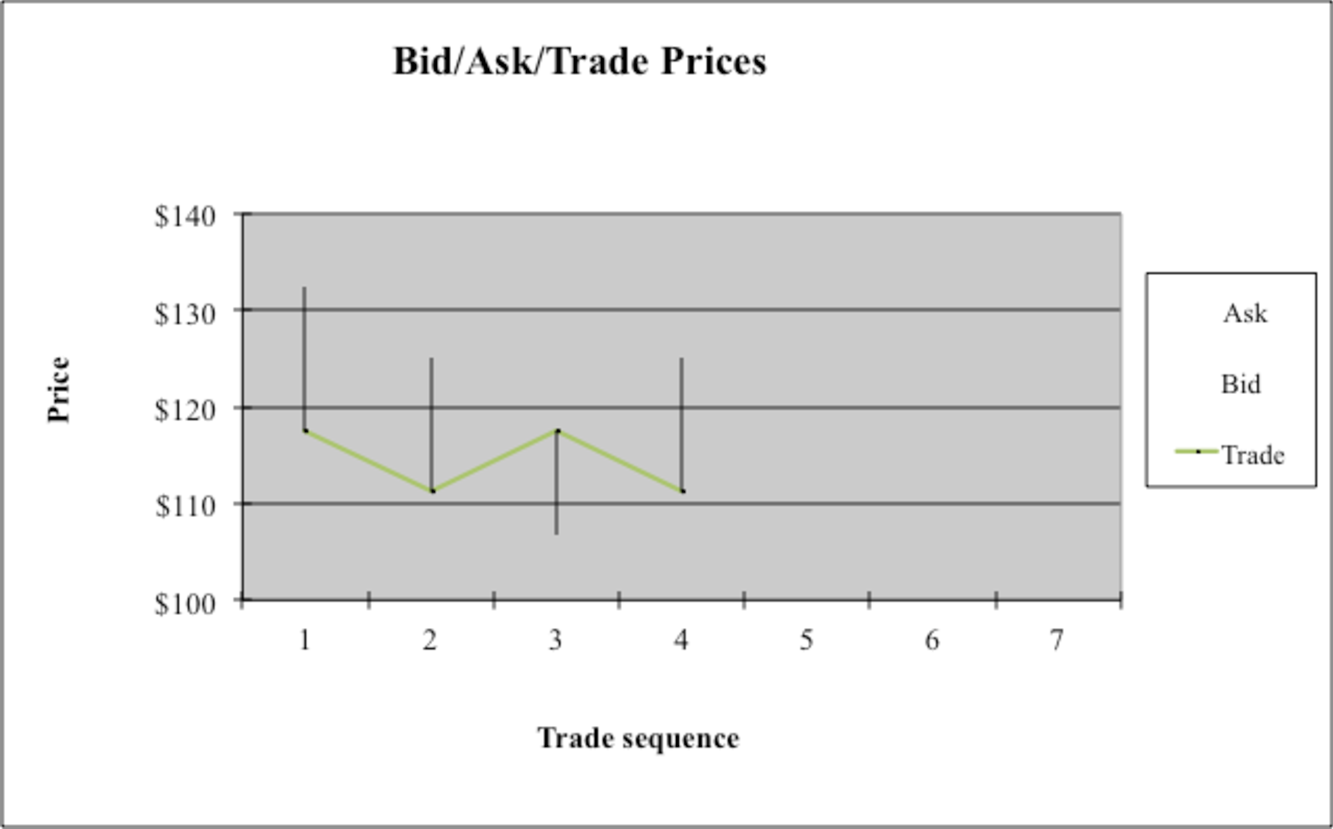
\includegraphics[width=0.9\linewidth]{pics/P4_Image.pdf}
\end{frame}


\begin{frame}<handout:0>{Dynamics}
	Fifth period: sell
	\center
	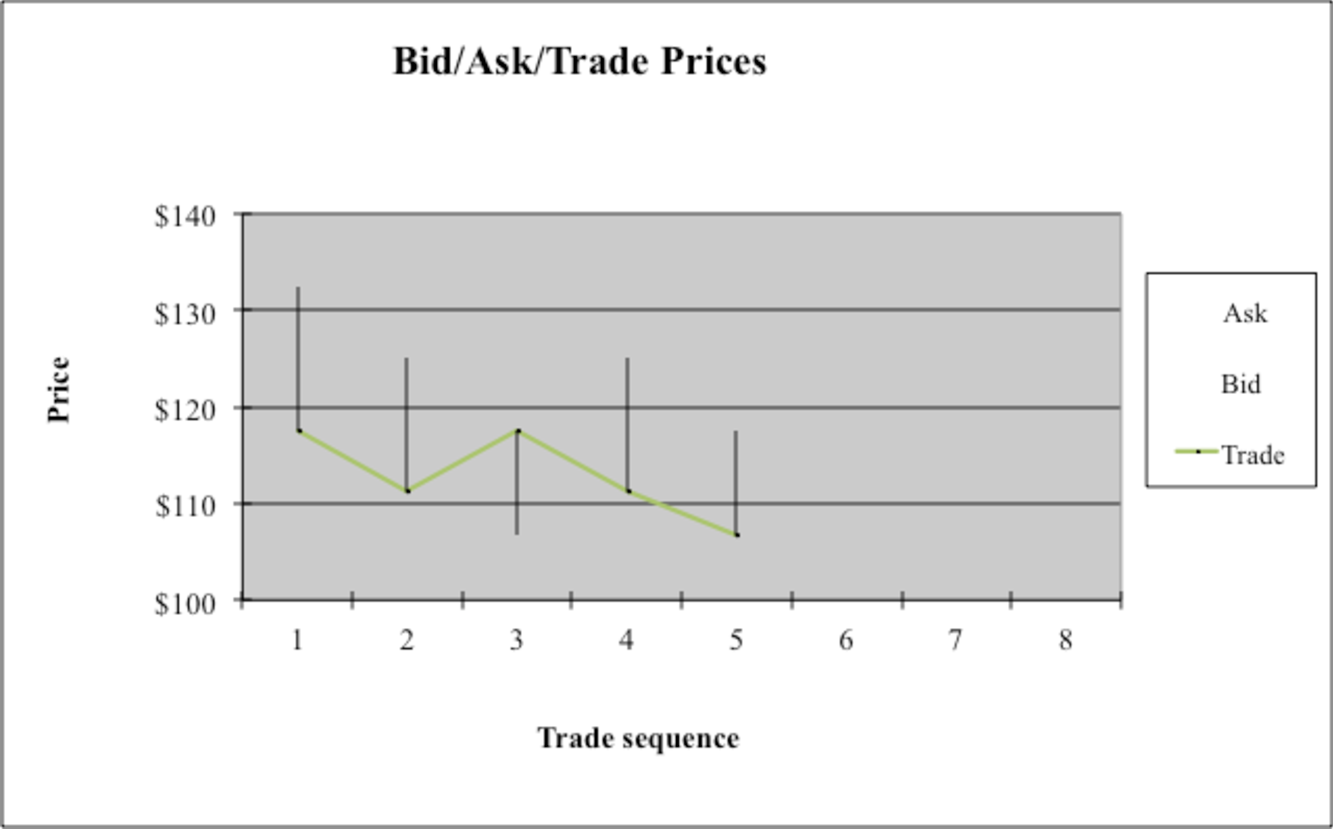
\includegraphics[width=0.9\linewidth]{pics/P5_Image.pdf}
\end{frame}


\begin{frame}<handout:0>{Dynamics}
	Sixth period: sell
	\center
	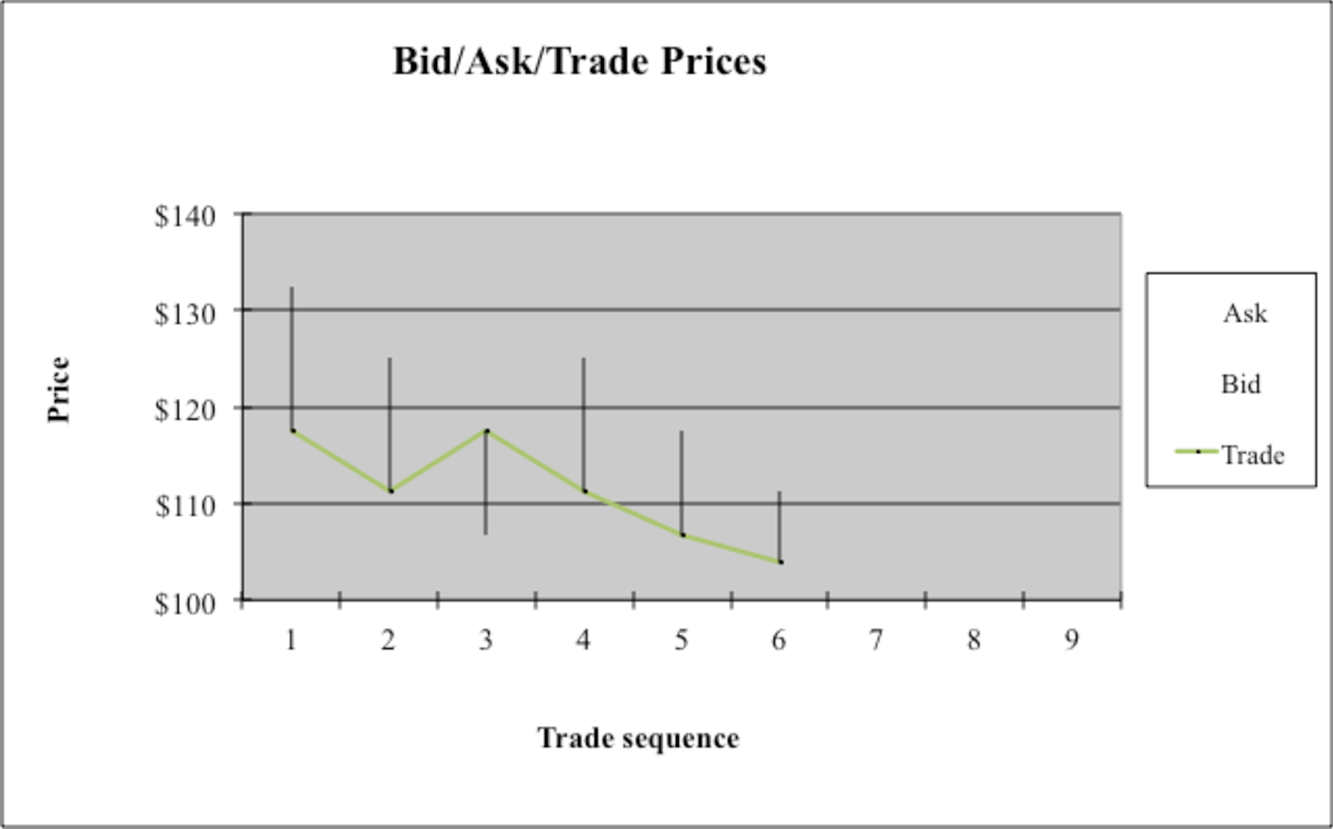
\includegraphics[width=0.9\linewidth]{pics/P6_Image.pdf}
\end{frame}


\begin{frame}<handout:0>{Dynamics}
	Seventh period: sell
	\center
	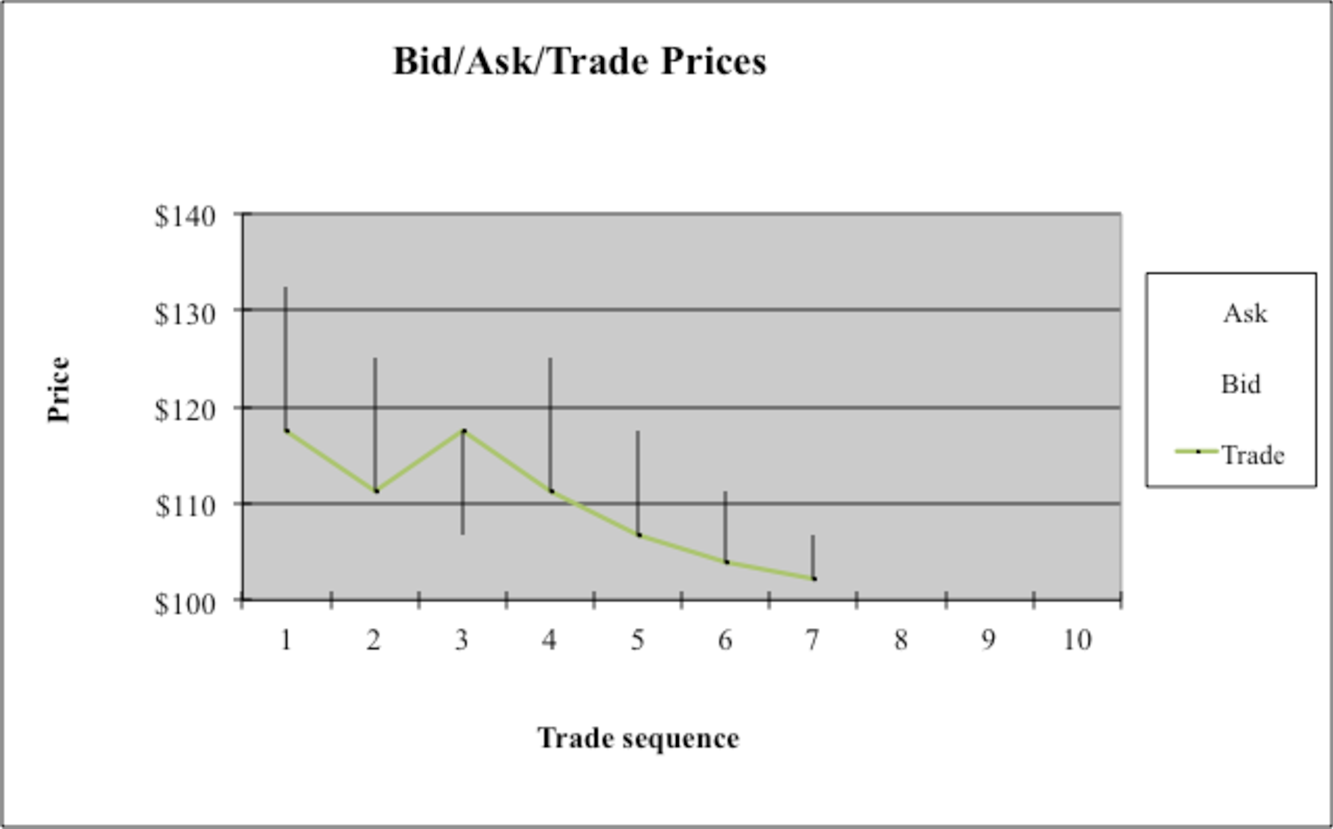
\includegraphics[width=0.9\linewidth]{pics/P7_Image.pdf}
\end{frame}


\begin{frame}<handout:0>{Dynamics}
	Eigth period: sell
	\center
	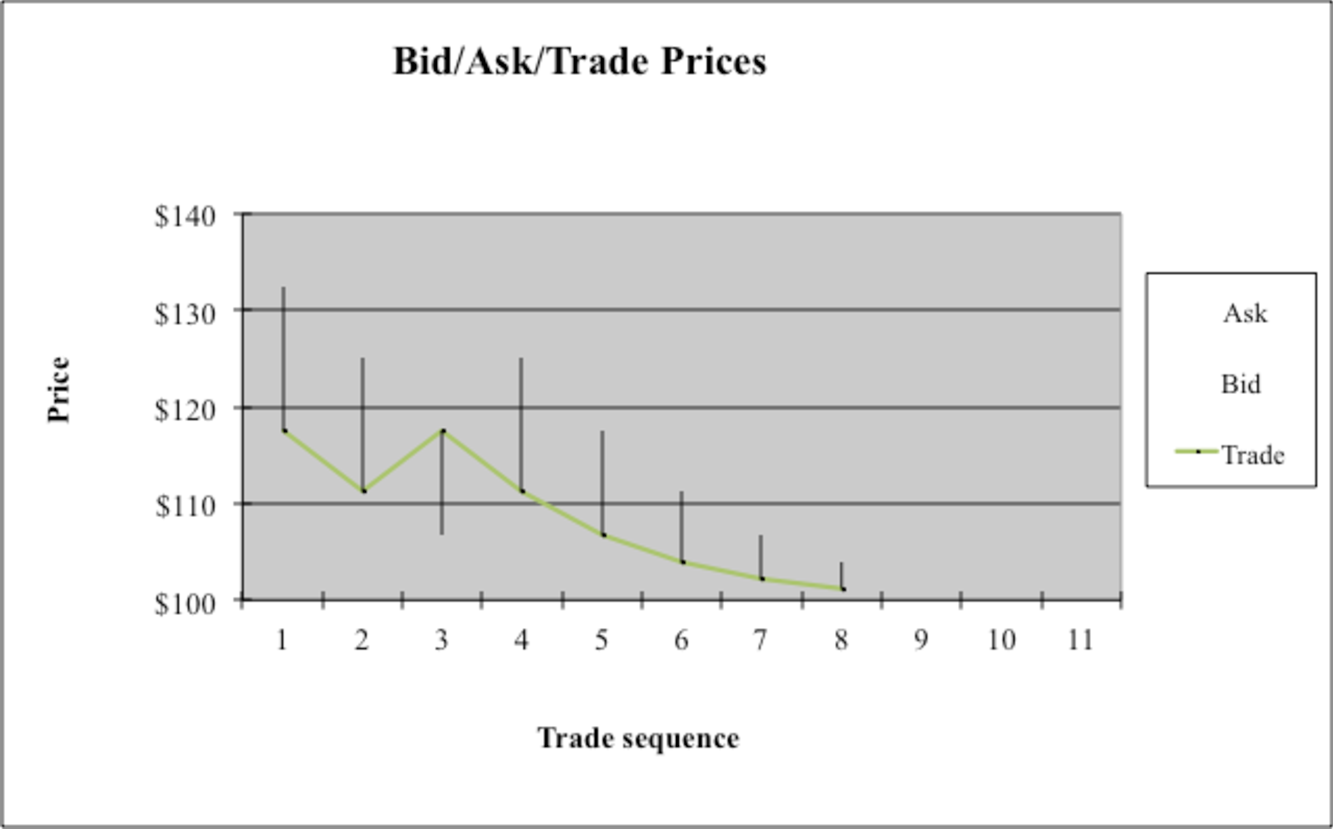
\includegraphics[width=0.9\linewidth]{pics/P8_Image.pdf}
\end{frame}


\begin{frame}<handout:0>{Dynamics}
	Ninth period: sell
	\center
	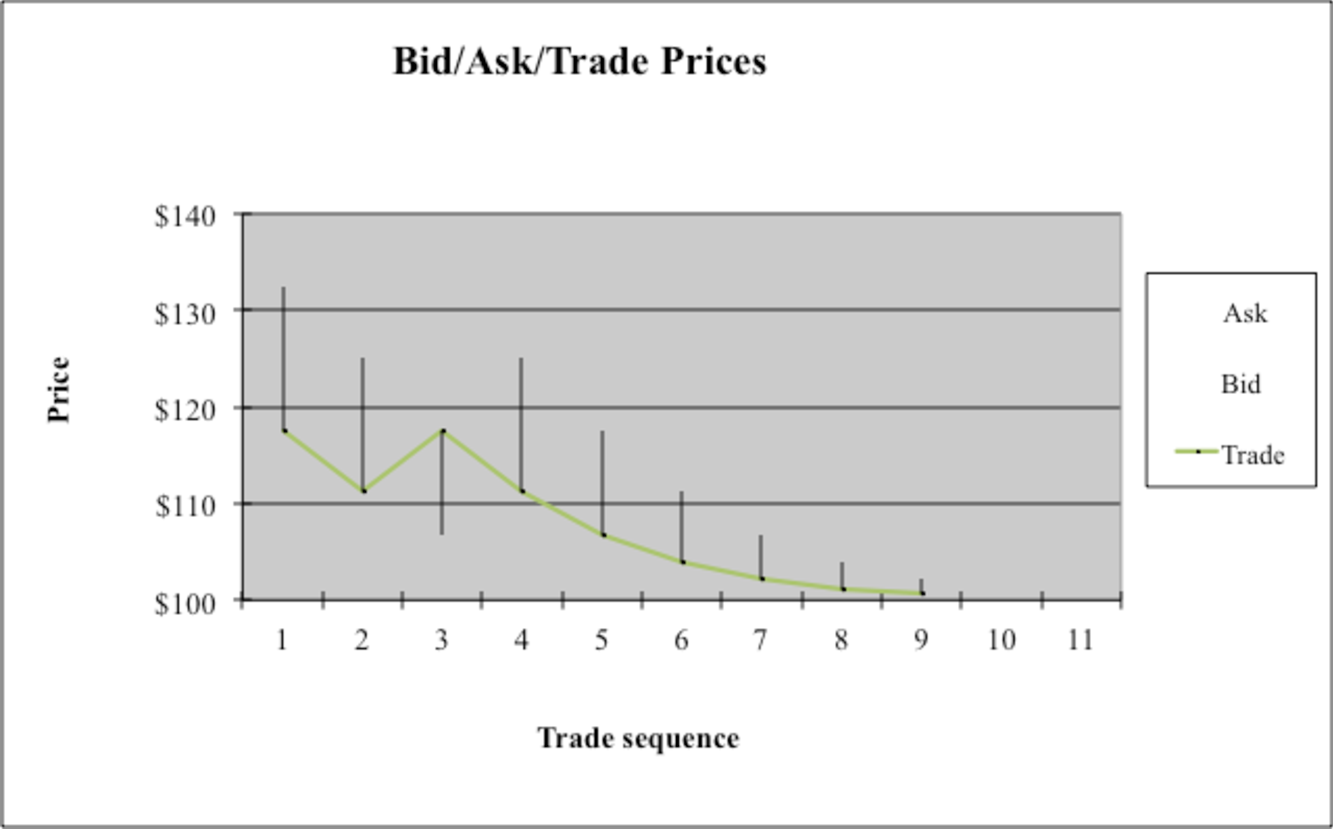
\includegraphics[width=0.9\linewidth]{pics/P9_Image.pdf}
\end{frame}


\begin{frame}<handout:0>{Dynamics}
	Tenth period: sell
	\center
	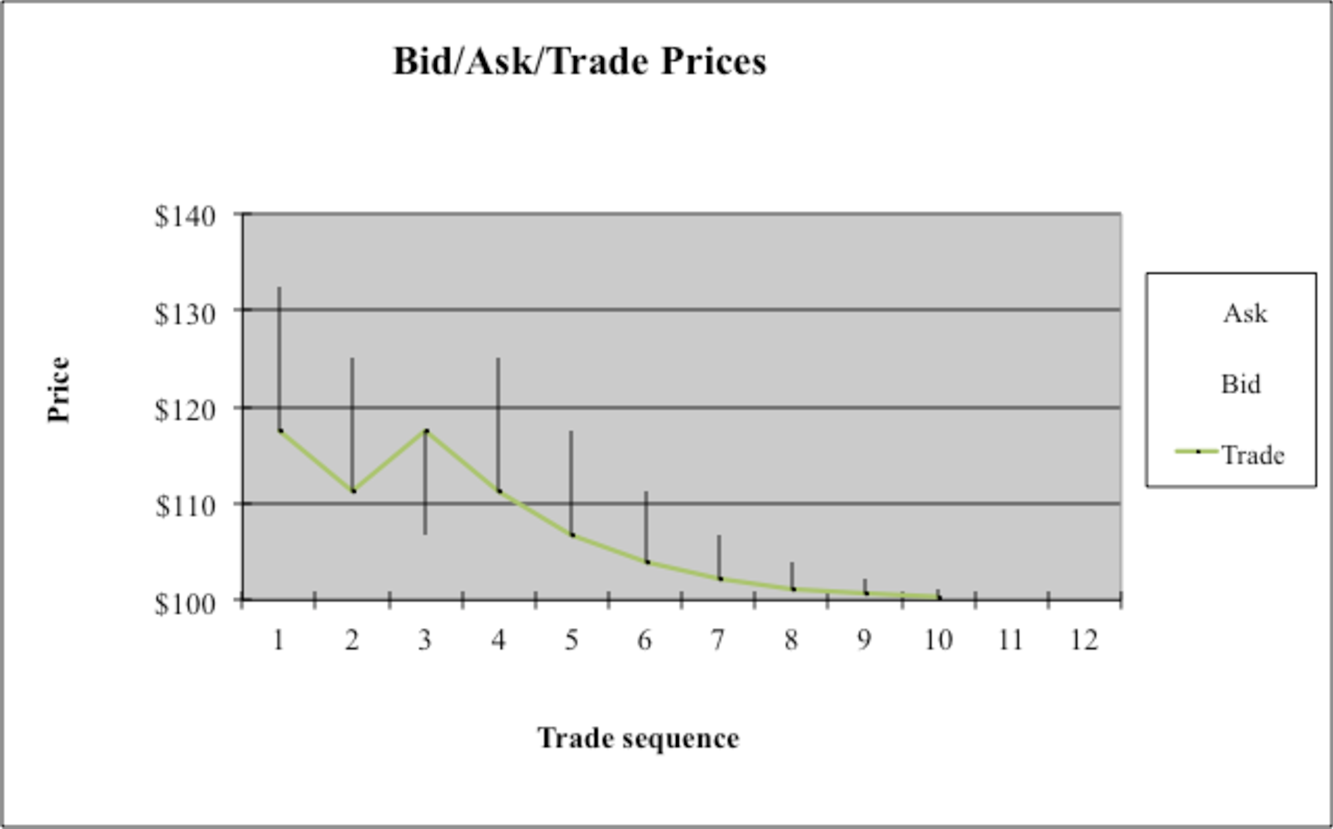
\includegraphics[width=0.9\linewidth]{pics/P10_Image.pdf}
\end{frame}


\begin{frame}<handout:0>{Dynamics}
	Eleventh period: sell
	\center
	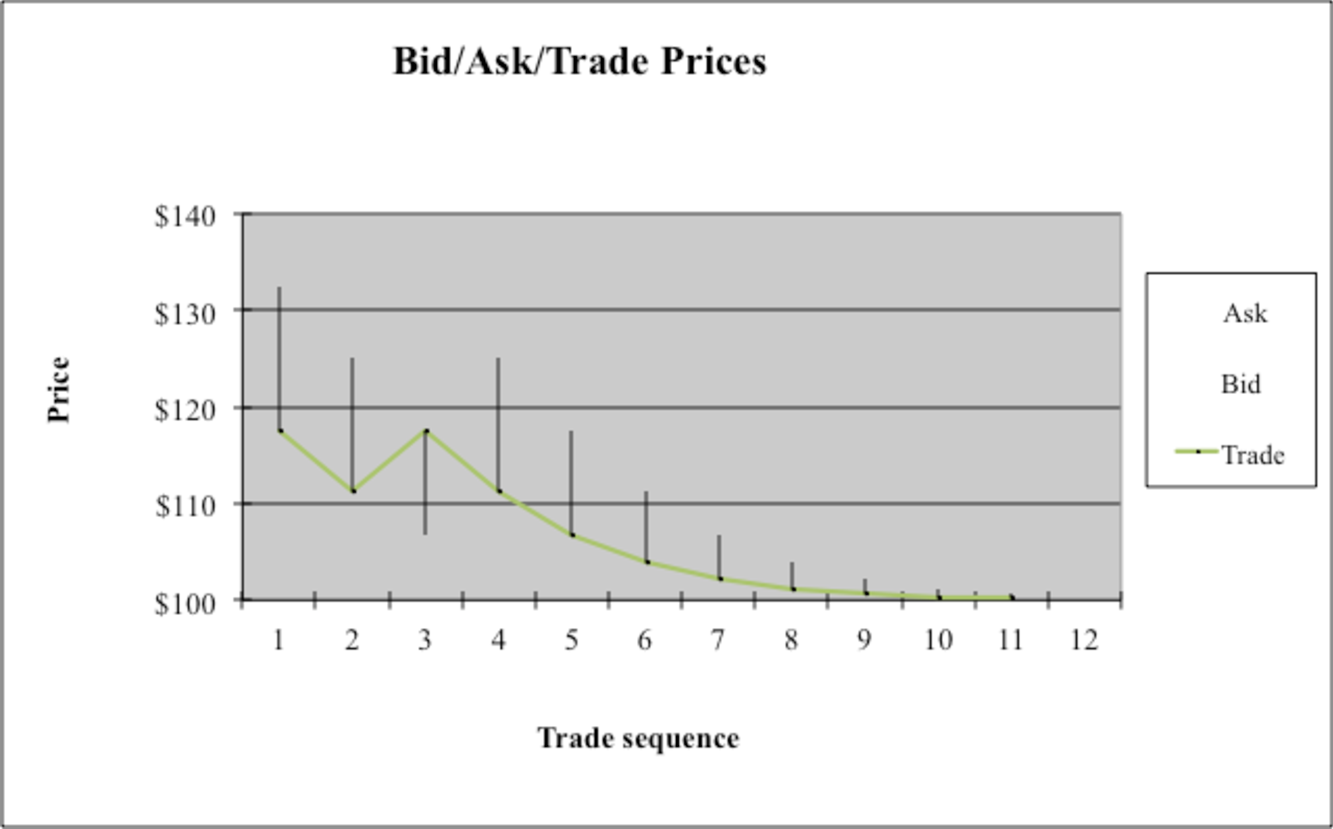
\includegraphics[width=0.9\linewidth]{pics/P11_Image.pdf}
\end{frame}


\begin{frame}{Dynamics}
	\only<handout:0>{Twelfth period: sell}
	\center
	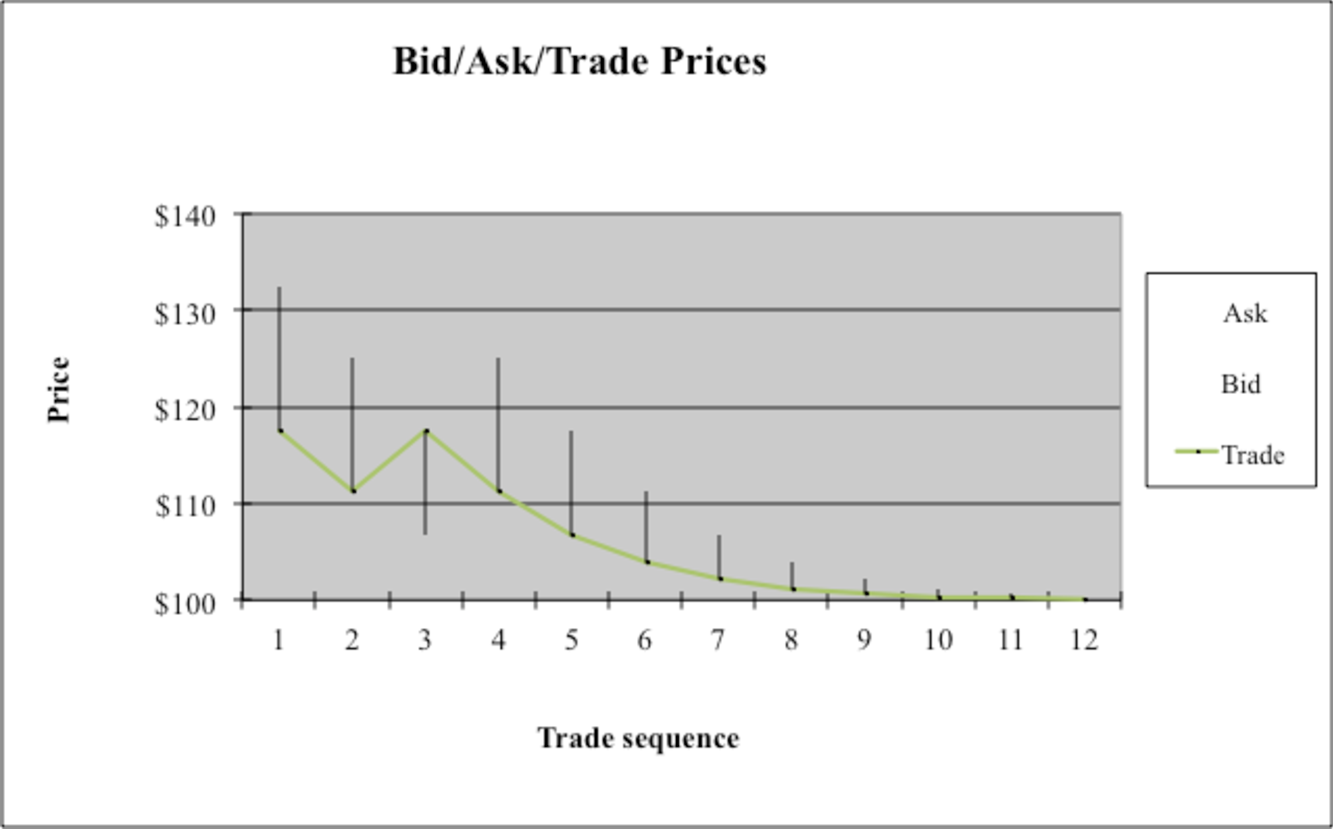
\includegraphics[width=0.9\linewidth]{pics/P12_Image.pdf}
\end{frame}


%\begin{frame}{Dynamics}
%	Let's consider an alternative case:
%	\[
%	bbbsssssssss
%	\]
%	Here we have a spell of buying in the beginning, before a long series of selling
%\end{frame}
%
%
%\begin{frame}{Dynamics}
%	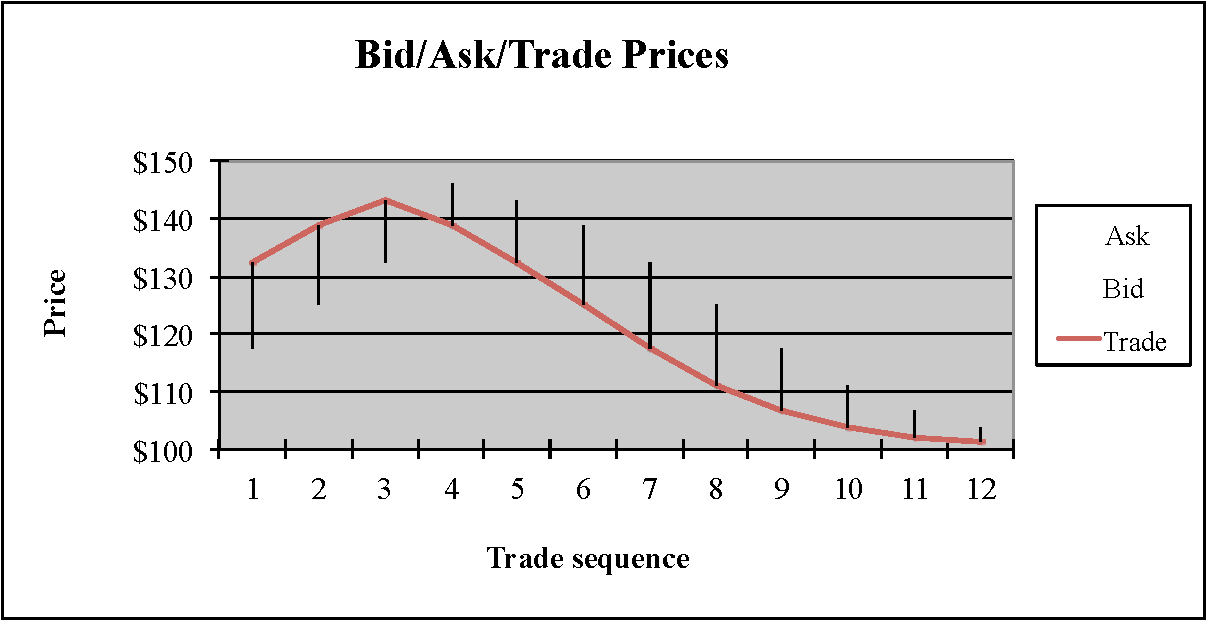
\includegraphics[width=1\linewidth]{pics/Bubble_Image.pdf}
%	\hyperlink{example}{\beamerbutton{back}}
%\end{frame}


\end{document} 